\begin{center}
{{\Large \sc High-Performance Computing}}
\end{center}
\rule{\textwidth}{1pt}
\begin{description}
\item[Student name and id:] % Marie Mørk \{s112770\} %Anders Launer Bæk \{s160159\} %\textcolor{red}{Marie Mørk \{s112770\} Anja Liljedahl Christensen\{s162876\}
 Andreas Vedel Jantzen \{s162858\}
 %Anders Launer Bæk \{s160159\}}
\item[Collaborators:] Anja Liljedahl Christensen\{s162876\} {Marie Mørk \{s112770\}} Anders Launer Bæk \{s160159\} %Andreas Vedel Jantzen \{s162858\} Anders Launer Bæk \{s160159\} {Marie Mørk \{s112770\} Anja Liljedahl Christensen\{s162876\}
 %Andreas Vedel Jantzen \{s162858\}
 %Anders Launer Bæk \{s160159\}}
\item[Hand-in:] GPU Computing
\end{description}
\rule{\textwidth}{1pt}

\section{Summary}
In the report, the problems from assignment 1 and 2 are solved by implementing algorithms that make use of GPUs. Six different algorithms for performing matrix multiplication are implemented. This includes a GPU library function. The performance of the algorithms are compared and a speed-up calculated using the cBLAS DGEMM subroutine as reference. The best performing algorithm is found to be \texttt{gpu5}, which one thread on the device to calculate each element in the resulting matrix $C$, and exploits shared memory. In the chosen range of problem sizes, this algorithm performs even better than the GPU library function, cublasDgemm. \\
Three Jacobi methods for solving the Poisson problem, with different levels of utilization of the GPU have also been implemented. The performance of these has been compared to the fastest CPU implementation from assignment 2. The best performing GPU implementation has a speed-up of $\approx \times 16$.

\section{Statement of the problem}
In this assignment GPU computing is used to solve the problems from the two earlier reports in order to see if GPU computing enhance the performance. The report is therefore split in two parts; one concerning matrix-matrix multiplication, and the other on the Poisson problem. \\ \ \\
\textbf{Matrix-matrix multiplication}\\
In the part about matrix-matrix multiplication, the dimensions of the matrices are the same as in Assignment 1, see figure \ref{fig:mat_or}. The performance of the implemented algorithms are to be compared with the cBLAS DGEMM subroutine used in Assignment 1. \\
\begin{figure}[H]
    \centering
    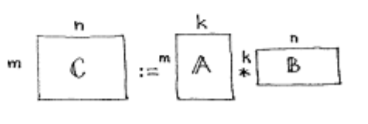
\includegraphics{contents/pics_1/matmult.PNG}
    \caption{Visualization of the matrix orientation. The picture is borrowed from the description of Assignment 1.}
    \label{fig:mat_or}
\end{figure}
\noindent Six different algorithms for matrix-matrix multiplications using GPUs are to be implemented. In the following, a short description of the algorithms is provided listed by their function calls. 
\begin{itemize}
    \item \texttt{lib}: Multithreaded cBLAS DGEMM subroutine as reference.
    \item \texttt{gpu1}: Using a single thread. 
    \item \texttt{gpu2}: Using one thread pr. element in matrix C.
    \item \texttt{gpu3}: Using one thread pr. 2 elements in matrix C. The optimal placement of the elements relative to each other is to be found.
    \item \texttt{gpu4}: Computing more than two elements in the C matrix pr. thread. The optimal placement of the elements relative to each other and number of elements is to be found.
    \item \texttt{gpu5}: Based upon the implementation linked to in the assignment description and modified to be compatible with the driver.
    \item \texttt{gpulib}: Implementation of the cuBLAS DGEMM subroutine.
\end{itemize} \ \\
\textbf{Poisson Problem}\\
The Poisson problem from assignment 2 will be solved using the Jacobi method. Three different algorithms will be implemented:
\begin{itemize}
    \item \texttt{jac\_cpu}: Best OpenMP function of the Jacobia function as reference.
    \item \texttt{jac\_gpu1}: A sequential version using one thread and doing one iteration pr kernel launch.
    \item \texttt{jac\_gpu2}: A naive version using one thread pr. grid point and only rely on global memory.
    \item \texttt{jac\_gpu3}: Multiple GPU version, in which the interior points are to be updated from global memory and the boarder points between the two regions is read as peer values from the other GPU.  
\end{itemize}
The kernels used are analyzed by the NVIDIA Visual Profiler (\texttt{nvvp}) in both parts of the assignment. 

\section{Hardware and software}
Specifications of the test environment are listed below:
\begin{itemize}
\item CPU information
\begin{itemize}
\item CPU(s):                24
\item Thread(s) per core:    1
\item Core(s) per socket:    12
\item Vendor ID:             GenuineIntel
\item CPU family:            6
\item Model:                 85
\item Model name:            Intel(R) Xeon(R) Gold 6126 CPU @ \item 2.60GHz
\item CPU MHz:               2600.000
\item L1 (d / i) cache:             32K
\item L2 cache:              1024K
\item L3 cache:              19712K
\end{itemize}

\item GPU information
\begin{itemize}
\item NVIDIA TESLA V100 FOR PCle x2
\item NVIDIA-SMI 387.26
\item Driver Version: 387.26
\end{itemize}
\item Compilers
\begin{itemize}
\item The SunCC compiler have been applied with followings flags: \texttt{-fast -xopenmp -xrestrict} for OpenMP reference in the Poisson problem.
\item \texttt{nnv} is used for default compilation of the cuda code.
\end{itemize}
\end{itemize}




\section{Theory}
%In this assignment a GPU will be used to solve problems, but why are GPUs important in HPC? For this to make sense lets go to the differences of how a GPU and a CPU process tasks. Very basic, a 
One of the advantages of using a GPU instead of a CPU is that while a CPU has few cores, a GPU has thousands of smaller more efficient cores, that can work simultaneously. This results in a much higher amount of floating point operations and a much higher bandwidth, though the GPU cores can only perform simple operations, and the CPU cores can be assigned to different and more complicated operations \cite{C4}.\\

\noindent The computations will be performed on a NVIDIA TESLA V100 GPU, hence the NVIDIA GPU optimized language CUDA will be used.\\

\noindent For medium to large matrices, matrix-matrix multiplication has the potential to be a compute-bound operation. The Jacobi method, on the other hand, is a memory-bound operation. %This report will examine the bounding, using the NVIDIA analysis tool \texttt{nvvp}. 

%Something on how the memory model works on GPUs and how this can be optimised. 

%Speed up

%Performance 

%SOmething about the nvvp profiler and how we use this

\newpage

\section{Matrix-matrix multiplication}
In this section the algorithms, results, and analysis of the kernels used for matrix-matrix multiplication will be presented. The performance of the algorithms will be compared with each other and the CBLAS library DGEMM subroutine, which was implemented in the function \texttt{matmult\_lib} in Assignment 1. The implementation of this algorithm will not be described again in this report, but the code is listed in the appendix, see algorithm \ref{alg:CPU_lib}.\\
Please note that the speed-ups are calculated based on the old driver on DTU Inside, which only uses 4 threads. Due to this, the calculated speed-ups are overestimated. Unfortunately, there was not sufficient time to update all the results.

\subsection{\texttt{gpu1}}
As already mentioned, in the implementation of \texttt{matmult\_gpu1} the kernel is launched with a single thread. The implementation of the algorithm (both the CPU function and the kernel) is listed in algorithm \ref{alg:gpu1}.\\

\lstinputlisting[label={alg:gpu1},caption={\texttt{matmult\_gpu1}, CPU function and kernel.},style=CStyle, 
linerange={21-73}]{code_3/func_cu.tex}

\noindent The performance of \texttt{matmult\_gpu1} will be compared to the CPU CBLAS subroutine DGEMM. Performance is only measured for small matrix sizes, in this case four square matrices of sizes N = M = K = 32, 64, 96, and 128. Figure \ref{fig:compare_gpu1} shows the number of floating point operations pr. second in Mflops/s for the four matrix sizes.\\

\noindent The figure shows that \texttt{matmult\_gpu1} is significantly slower than the optimized CPU library function DGEMM. This is as expected, as the GPU version only uses one thread, which means that the version is sequential and thereby does not take advantage of parallelism of the threads in the GPU. In addition to this, \texttt{gpu1} uses time for copying memory between the host and the device. The CPU function implementation on the other hand, is optimized using parallel programming ect. which makes it much faster. \\

\noindent In figure \ref{fig:speed_gpu1}, the speed-up of \texttt{gpu1} compared to \texttt{lib} is shown. As it is already apparent from figure \ref{fig:compare_gpu1}, the speed-up is below 1, meaning that the CPU version is faster than the GPU. \\

\noindent Performance of the GPUs is also evaluated using the \texttt{nvprof} command in the shell. For \texttt{gpu1}, the GPU summary shows that $99.98\%-100\%$ of the time used for executing the GPU function is used in the kernel, whereas very little time is used for copying between host and device. This shows that in order for the algorithm to have a better performance, the computations within the kernels should be optimized. \\


\begin{figure}[H]
\centering
\begin{tikzpicture}[scale = 0.85]
\begin{axis}[
width=17cm, height=8cm,     % size of the image
grid = major,
grid style={dashed, gray!30},
xmode=log,log basis x=10,
%ymin=0,    % start the diagram at this 
%ymax=155000, % end   the diagram at this 
axis background/.style={fill=white},
ylabel=Mflops/s,
xlabel=Memory/kbytes,
legend pos=north west]
\addplot[mark=*, orange] table [x=mem, y=mflops, col sep=comma]{data_3/mat/lib_small.txt};
\addlegendentry{\texttt{lib()}}
\addplot[mark=*, blue] table [x=mem, y=mflops, col sep=comma]{data_3/mat/gpu1.txt};
\addlegendentry{\texttt{gpu1()}}
\end{axis} 
\end{tikzpicture}
\caption{Comparison of \texttt{gpu1} and \texttt{lib}.}
\label{fig:compare_gpu1}
\end{figure}

\begin{figure}[H]
\centering
\begin{tikzpicture}[scale = 0.85]
\begin{axis}[
width=17cm, height=8cm,     % size of the image
grid = major,
grid style={dashed, gray!30},
xmode=log,log basis x=10,
%ymin=0,    % start the diagram at this 
%ymax=155000, % end   the diagram at this 
axis background/.style={fill=white},
ylabel=Speed-up,
xlabel=Memory/kbytes,
legend pos=north west]
\addplot[mark=*, orange] table [x=mem, y=speed, col sep=comma]{data_3/mat/speed_gpu1.txt};
\addlegendentry{Speed-up}
\end{axis} 
\end{tikzpicture}
\caption{Speed up of \texttt{gpu1} compared to \texttt{lib}.}
\label{fig:speed_gpu1}
\end{figure}


\subsection{\texttt{gpu2}}
The kernel for \texttt{matmult\_gpu2} is listed in algorithm \ref{alg:gpu2K}, while the changes in the launch from the CPU function is listed in \ref{alg:gpu2L}. This time each thread computes one element of $C$: the thread with global thread id $(i,j)$ computes element $(i,j)$ in $C$. If there are more threads than elements in $C$ the remaining threads will not compute anything.\\

\lstinputlisting[label={alg:gpu2K},caption={\texttt{matmult\_gpu2} kernel.},style=CStyle, linerange={76-89}]{code_3/func_cu.tex}
\lstinputlisting[label={alg:gpu2L},caption={\texttt{matmult\_gpu2} launch of kernel.},style=CStyle, linerange={111-114}]{code_3/func_cu.tex}

\noindent Matrix sizes used for the comparison between \texttt{gpu2} and the CPU library function is set to be multiples of 16, such that the same matrix sizes can be used to compare with \texttt{gpu5} in a later section. We choose square matrices with dimensions 800, 1600, 2400, 3200, 4000, 4800, and 5600. In figure \ref{fig:compare_gpu2}, Mflops/s as a function of problem size is shown for \texttt{gpu2} and \texttt{lib}. Comparing the two graphs, the advantages of using GPUs is now clearly visible and \texttt{gpu2} is faster than \texttt{lib} for all matrix sizes considered. \\
\begin{figure}[H]
\centering
\begin{tikzpicture}[scale = 0.85]
\begin{axis}[
width=17cm, height=8cm,     % size of the image
grid = major,
grid style={dashed, gray!30},
xmode=log,log basis x=10,
%ymin=0,    % start the diagram at this 
%ymax=155000, % end   the diagram at this 
axis background/.style={fill=white},
ylabel=Mflops/s,
xlabel=Memory/kbytes,
legend pos=north west]
\addplot[mark=*, orange] table [x=mem, y=mflops, col sep=comma]{data_3/mat/lib.txt};
\addlegendentry{\texttt{lib()}}
\addplot[mark=*, blue] table [x=mem, y=mflops, col sep=comma]{data_3/mat/gpu2.txt};
\addlegendentry{\texttt{gpu2()}}
\end{axis} 
\end{tikzpicture}
\caption{Comparison of \texttt{gpu2} and \texttt{lib}.}
\label{fig:compare_gpu2}
\end{figure}
\noindent The speed-up is computed from mflops/s and reported in figure \ref{fig:speed_gpu2} for the chosen matrix sizes. It is seen that the speed-up rises with problem size up until matrices with dimensions higher than 3200. For larger matrices, the speed-up stays constant at around 4x. 

\begin{figure}[H]
\centering
\begin{tikzpicture}[scale = 0.85]
\begin{axis}[
width=17cm, height=8cm,     % size of the image
grid = major,
grid style={dashed, gray!30},
xmode=log,log basis x=10,
%ymin=0,    % start the diagram at this 
%ymax=155000, % end   the diagram at this 
axis background/.style={fill=white},
ylabel=Speed-up,
xlabel=Memory/kbytes,
legend pos=north west]
\addplot[mark=*, orange] table [x=mem, y=speed, col sep=comma]{data_3/mat/speed_gpu2.txt};
\addlegendentry{Speed-up}
\end{axis} 
\end{tikzpicture}
\caption{Speed up of \texttt{gpu2} compared to \texttt{lib}.}
\label{fig:speed_gpu2}
\end{figure}

\noindent Using the call \texttt{nvprof --print-gpu-summary} in the shell, the different parts of the GPU function is timed. In table \ref{tab:time_gpu2}, the percentage used in the kernel, on copying from host to device, and from device to host is listed. For smaller problem sizes, the percentage of the total execution time used in the kernel is smaller than for large problems. It is to expect, as fewer calculations are needed for small matrices, while the memory still needs to be transferred between host and device.

\begin{table}[H]
    \centering
    \begin{tabular}{c|c c c}
         Problem size&Kernel & HtoD & DtoH \\ \hline
         800 & 81.63\% & 12.55\% & 5.82\% \\
         1600 & 89.86\% & 6.92\% & 3.23\% \\
         2400 & 92.93\% & 4.82\% & 2.25\% \\
         3200 & 94.11\% & 4.01\% & 1.88\% \\
         4000 &95.19\% & 3.28\% & 1.53\%\\
         4800 & 95.95\% & 2.76\% & 1.29\% \\
         5600 & 96.51\% & 2.38\%& 1.11\%
    \end{tabular}
    \caption{Time spend on Kernel, HtoD and DtoH in the kernel of \texttt{gpu2} for the chosen problem sizes.}
    \label{tab:time_gpu2}
\end{table}

\subsection{\texttt{gpu3}}
In \texttt{gpu3}, each thread is to compute 2 elements in $C$. To do this, a stride introduced in the algorithm. The function is tested for the stride in both the $x$ and the $y$ direction for large matrices. A stride in $y$ is found to be the fastest, hence the second element in $C$ which is computed by the thread is the neighbor below the first element. This makes sense since in this way the threads access memory coalesced. Furthermore this way a single thread will access one column in $B$ and two rows in $A$ in order to compute the two elements in $C$. As memory storage in $C$ is row-major, it is expected that accessing two rows and one column is faster than the opposite for each thread. The kernel for this implementation is listed in algorithm \ref{alg:gpu3K}, while the changes in the launch from the CPU function is listed in algorithm \ref{alg:gpu3L}.\\
\noindent Compared to the previous two kernels \texttt{gpu3\_kernel} takes an extra argument which is the stride in the $y$ ($i$) direction. Since each thread has to compute 2 elements, \texttt{stride} is set to 2 when the kernel is launched, see algorithm \ref{alg:gpu3L}. In algorithm \ref{alg:gpu3K} the thread with global thread id $(i,j)$ will then compute element $(i\cdot 2, j)$ and $(i\cdot 2 + 1, j)$ of $C$. \\

\lstinputlisting[label={alg:gpu3K},caption={\texttt{gpu3} kernel.},style=CStyle, linerange={132-147}]{code_3/func_cu.tex}
\lstinputlisting[label={alg:gpu3L},caption={\texttt{gpu3} launch of kernel.},style=CStyle, linerange={170-173}]{code_3/func_cu.tex}

\noindent Again, the performance of the algorithm is compared to that of \texttt{lib}. In figure \ref{fig:compare_gpu3}, Mflops/s is shown for different problem sizes. For the largest problem size, \texttt{gpu3} computes almost twice as many Mflops/s as \texttt{gpu2}. This means that the speed up compared to the CPU version is higher for \texttt{gpu3}.
\begin{figure}[H]
\centering
\begin{tikzpicture}[scale = 0.85]
\begin{axis}[
width=17cm, height=8cm,     % size of the image
grid = major,
grid style={dashed, gray!30},
xmode=log,log basis x=10,
%ymin=0,    % start the diagram at this 
%ymax=155000, % end   the diagram at this 
axis background/.style={fill=white},
ylabel=Mflops/s,
xlabel=Memory/kbytes,
legend pos=north west]
\addplot[mark=*, orange] table [x=mem, y=mflops, col sep=comma]{data_3/mat/lib.txt};
\addlegendentry{\texttt{lib()}}
\addplot[mark=*, blue] table [x=mem, y=mflops, col sep=comma]{data_3/mat/gpu3.txt};
\addlegendentry{\texttt{gpu3()}}
\end{axis} 
\end{tikzpicture}
\caption{Comparison of \texttt{gpu3} and \texttt{lib}.}
\label{fig:compare_gpu3}
\end{figure}

\noindent In figure \ref{fig:speed_gpu3}, the calculated speed-ups are shown for the chosen problem sizes. The graph shows the same tendency as the speed-up for \texttt{gpu2} namely that the speed up cease to increase for problem sizes larger than 3200. The speed-up is almost doubled compared to \texttt{gpu2}.

\begin{figure}[H]
\centering
\begin{tikzpicture}[scale = 0.85]
\begin{axis}[
width=17cm, height=8cm,     % size of the image
grid = major,
grid style={dashed, gray!30},
xmode=log,log basis x=10,
%ymin=0,    % start the diagram at this 
%ymax=155000, % end   the diagram at this 
axis background/.style={fill=white},
ylabel=Speed-up,
xlabel=Memory/kbytes,
legend pos=north west]
\addplot[mark=*, orange] table [x=mem, y=speed, col sep=comma]{data_3/mat/speed_gpu3.txt};
\addlegendentry{Speed-up}
\end{axis} 
\end{tikzpicture}
\caption{Speed up of \texttt{gpu3} compared to \texttt{lib}.}
\label{fig:speed_gpu3}
\end{figure}

\subsection{\texttt{gpu4}}
In the previous version each thread computed 2 elements of $C$, but now the number of elements for each thread has to be more than 2. It is immediately ruled out to assign elements in more than 1 column of $C$ for each thread (since it is faster for the threads to access memory coalesced), hence the question is: how many element in 1 column (directly on top of each other) should each thread compute. This is investigated by using the matrix sizes $M=N=K=5000$ and trying out different strides in the $y$ direction. The kernel is listed in algorithm \ref{alg:gpu4K}, while the changes in the launch from the CPU function is listed in algorithm \ref{alg:gpu4L}.\\

\lstinputlisting[label={alg:gpu4K},caption={\texttt{gpu4} kernel.},style=CStyle, linerange={191-212}]{code_3/func_cu.tex}
\lstinputlisting[label={alg:gpu4L},caption={\texttt{gpu4} launch of kernel.},style=CStyle, linerange={235-238}]{code_3/func_cu.tex}

\noindent In figure \ref{fig:gpu4_opt} below the GPU time is recorded for small values of \texttt{stride\_m}, i.e. from 3 to 64, and in figure \ref{fig:gpu4_opt2} the GPU time is recorded for larger values of \texttt{stride\_m}. The size of both strides (\texttt{stride\_n} in the $x$ direction and \texttt{stride\_m} in the $y$ direction) are given as arguments from the command line. This might explain the strange behavior of the GPU time. When the strides are not predefined at compile time, memory is not allocated optimally. Hence, the registers of the threads are not fully exploited. From the plots below, the GPU time is minimal when each thread computes 6 elements, though it is hard to see.  

\begin{figure}[H]
\centering
\begin{tikzpicture}[scale = 0.85]
\begin{axis}[
width=17cm, height=8cm,     % size of the image
grid = major,
grid style={dashed, gray!30},
%xmode=log,log basis x=10,
ymin=0.6,    % start the diagram at this 
ymax=1.35, % end   the diagram at this 
axis background/.style={fill=white},
ylabel=Time in s.,
xlabel=stride\_m,
legend pos=north west]
\addplot[mark=*, orange] table [x=stride_m, y=time, col sep=comma]{data_3/gpu4_opt2.txt};
%\addlegendentry{\texttt{lib()}}
% \addplot[mark=*, blue] table [x=mem, y=mflops, col sep=comma]{data_3/mat/gpu1.txt};
%\addlegendentry{\texttt{gpu4()}}
\end{axis} 
\end{tikzpicture}
\caption{GPU time for \texttt{matmult\_gpu4} for different small sizes of \texttt{stride\_m}.}
\label{fig:gpu4_opt}
\end{figure}

\begin{figure}[H]
\centering
\begin{tikzpicture}[scale = 0.85]
\begin{axis}[
width=17cm, height=8cm,     % size of the image
grid = major,
grid style={dashed, gray!30},
%xmode=log,log basis x=10,
ymin=0.6,    % start the diagram at this 
ymax=1.35, % end   the diagram at this 
axis background/.style={fill=white},
ylabel=Time in s.,
xlabel=stride\_m,
legend pos=north west]
\addplot[mark=*, orange] table [x=stride_m, y=time, col sep=comma]{data_3/gpu4_opt.txt};
%\addlegendentry{\texttt{lib()}}
% \addplot[mark=*, blue] table [x=mem, y=mflops, col sep=comma]{data_3/mat/gpu1.txt};
%\addlegendentry{\texttt{gpu4()}}
\end{axis} 
\end{tikzpicture}
\caption{GPU time for \texttt{matmult\_gpu4} for different large sizes of \texttt{stride\_m}.}
\label{fig:gpu4_opt2}
\end{figure}

\noindent Below in algorithm \ref{alg:gpu4Kopt} is the altered kernel for \texttt{matmult\_gpu4} where the outer stride for-loop has been removed (since \texttt{stride\_n} is always chosen to be 1), and the variable \texttt{stride\_m} has been replaced by a fixed integer (6 in this case). This means that both the kernel and \texttt{matmult\_gpu4} take 2 arguments less than the original versions.\\

\noindent "Hardcoding" the stride for different sizes did surprisingly and unfortunately not result in better GPU times, and $\texttt{stride\_m} = 6$ is still the optimal choice.\\

\lstinputlisting[label={alg:gpu4Kopt},caption={Optimized \texttt{gpu4} kernel.},style=CStyle, linerange={1-17}]{code_3/opt_gpu4_kernel.c}

\noindent In figure \ref{fig:compare_gpu4} below the number of floating points operations per second of \texttt{matmult\_gpu4} is compared to \texttt{matmult\_gpu3} and \texttt{matmult\_lib}, and in figure \ref{fig:speed_gpu4} the speed-up of \texttt{matmult\_gpu4} is compared to \texttt{matmult\_gpu3}. The efficiency of \texttt{matmult\_gpu4} is actually worse than the efficiency of the previous version, i.e. according to the implementations of these kernel-functions the best efficiency and speed-up is achieved when each thread computes 2 elements of $C$ instead of 1 or $>2$. This is not as expected and is probably also due to the above issue with memory allocation at compile time. 

\begin{figure}[H]
\centering
\begin{tikzpicture}[scale = 0.85]
\begin{axis}[
width=17cm, height=8cm,     % size of the image
grid = major,
grid style={dashed, gray!30},
xmode=log,log basis x=10,
%ymin=0,    % start the diagram at this 
%ymax=155000, % end   the diagram at this 
axis background/.style={fill=white},
ylabel=Mflops/s,
xlabel=Memory/kbytes,
legend pos=north west]
\addplot[mark=*, orange] table [x=mem, y=mflops, col sep=comma]{data_3/mat/lib.txt};
\addlegendentry{\texttt{lib()}}
\addplot[mark=*, blue] table [x=mem, y=mflops, col sep=comma]{data_3/mat/gpu3.txt};
\addlegendentry{\texttt{gpu3()}}
\addplot[mark=*, green] table [x=mem, y=mflops, col sep=comma]{data_3/mat/gpu4.txt};
\addlegendentry{\texttt{gpu4()}}
\end{axis} 
\end{tikzpicture}
\caption{Comparison of \texttt{gpu4} and \texttt{lib}.}
\label{fig:compare_gpu4}
\end{figure}

\begin{figure}[H]
\centering
\begin{tikzpicture}[scale = 0.85]
\begin{axis}[
width=17cm, height=8cm,     % size of the image
grid = major,
grid style={dashed, gray!30},
xmode=log,log basis x=10,
%ymin=0,    % start the diagram at this 
%ymax=155000, % end   the diagram at this 
axis background/.style={fill=white},
ylabel=Speed-up,
xlabel=Memory/kbytes,
legend pos=north west]
\addplot[mark=*, red] table [x=mem, y=speed, col sep=comma]{data_3/mat/speed_gpu4.txt};
\addlegendentry{Speed-up of \texttt{gpu4}}
\addplot[mark=*, orange] table [x=mem, y=speed, col sep=comma]{data_3/mat/speed_gpu3.txt};
\addlegendentry{Speed-up of \texttt{gpu3}}
\end{axis} 
\end{tikzpicture}
\caption{Speed up of \texttt{gpu4} compared to \texttt{lib}.}
\label{fig:speed_gpu4}
\end{figure}

\subsection{\texttt{gpu5}}
The \texttt{gpu5} version is based on the shared memory matrix-matrix multiplication algorithm given on \url{http://docs.nvidia.com/cuda/cuda-c-programming-guide/index.html#shared-memory}. Several things had to be changed in order for this version to be compatible with the driver and for it to provide the correct result. \textbf{Please note} that since the original version assumes that $M$, $N$, and $K$ are integer multiples of the block thread size (i.e. $16\times 16$), the modified version also assumes that $M$, $N$, and $K$ are multiples of 16.\\

\noindent The issue with the compatibility is solved by simply changing the input arguments of \texttt{matmult\_gpu5}. This means that the way the matrices $A$, $B$ and $C$ are loaded to the device memory also has to be changed. This is done by using the matrix sizes $M$, $N$, and $K$ directly as well as the matrices $A$, $B$, and $C$, instead of first creating a Matrix struct for each of the host matrices and then use these to create the device Matrix structs. The modified version is given in algorithm \ref{alg:gpu5L} below.\\

\noindent Lastly all variables and help functions of type \texttt{float} have to be changed to \texttt{double} such that there are no round-off errors.\\

\lstinputlisting[label={alg:gpu5L},caption={\texttt{gpu4} launch of kernel.},style=CStyle, linerange={399-434}]{code_3/func_cu.tex}

\noindent In figure \ref{fig:compare_gpu5} the efficiency of this version is compared to the dgemm subroutine. This is by far the fastest version and contrary to the previous versions Mflops/s is increased linearly with the problem size. The improvement of the fifth version is also especially evident when considering the speed-up compared to the dgemm subroutine in figure \ref{fig:speed_gpu5}. With version three the maximal speed-up was close to 8 but version five the maximal speed-up is almost 30.

\begin{figure}[H]
\centering
\begin{tikzpicture}[scale = 0.85]
\begin{axis}[
width=17cm, height=8cm,     % size of the image
grid = major,
grid style={dashed, gray!30},
xmode=log,log basis x=10,
%ymin=0,    % start the diagram at this 
%ymax=155000, % end   the diagram at this 
axis background/.style={fill=white},
ylabel=Mflops/s,
xlabel=Memory/kbytes,
legend pos=north west]
\addplot[mark=*, orange] table [x=mem, y=mflops, col sep=comma]{data_3/mat/lib.txt};
\addlegendentry{\texttt{lib()}}
\addplot[mark=*, blue] table [x=mem, y=mflops, col sep=comma]{data_3/mat/gpu5.txt};
\addlegendentry{\texttt{gpu5()}}
\end{axis} 
\end{tikzpicture}
\caption{Comparison of \texttt{gpu5} and \texttt{lib}.}
\label{fig:compare_gpu5}
\end{figure}

\begin{figure}[H]
\centering
\begin{tikzpicture}[scale = 0.85]
\begin{axis}[
width=17cm, height=8cm,     % size of the image
grid = major,
grid style={dashed, gray!30},
xmode=log,log basis x=10,
%ymin=0,    % start the diagram at this 
%ymax=155000, % end   the diagram at this 
axis background/.style={fill=white},
ylabel=Speed-up,
xlabel=Memory/kbytes,
legend pos=north west]
\addplot[mark=*, orange] table [x=mem, y=speed, col sep=comma]{data_3/mat/speed_gpu5.txt};
\addlegendentry{Speed-up}
\end{axis} 
\end{tikzpicture}
\caption{Speed up of \texttt{gpu5} compared to \texttt{lib}.}
\label{fig:speed_gpu5}
\end{figure}

\subsection{\texttt{gpulib}}
The last matrix multiplication algorithm is the DGEMM function for GPUs that has been implemented in the function \texttt{gpulib} such that it can be run on the provided driver. The cublasDgemm function takes 14 arguments and is column-major. The matrix A and its LDA the matrix B and its LDB have been swooped in order to make cublasDgemm row-major. The implemented function is listed in algo. \ref{alg:gpuLIB}. \\

\lstinputlisting[label={alg:gpuLIB},caption={\texttt{gpulib} launch of kernel.},style=CStyle, linerange={257-300}]{code_3/func_cu.tex}


\noindent In figure \ref{fig:compare_gpulib}, the number of floating point operations performed pr second is shown for different problem sizes. For small problem sizes, the CPU version of DGEMM, \texttt{lib} is faster than the GPU version, \texttt{gpulib}. This changes for matrices with dimensions a little larger than 1600, for which the GPU version becomes faster. Figure \ref{fig:speed_gpulib} shows the speed-up for the chosen problem sizes. As was the case with \texttt{gpu5}, the speed-up does not wear off for large problem sizes. 

\begin{figure}[H]
\centering
\begin{tikzpicture}[scale = 0.85]
\begin{axis}[
width=17cm, height=8cm,     % size of the image
grid = major,
grid style={dashed, gray!30},
xmode=log,log basis x=10,
%ymin=0,    % start the diagram at this 
%ymax=155000, % end   the diagram at this 
axis background/.style={fill=white},
ylabel=Mflops/s,
xlabel=Memory/kbytes,
legend pos=north west]
\addplot[mark=*, orange] table [x=mem, y=mflops, col sep=comma]{data_3/mat/lib.txt};
\addlegendentry{\texttt{lib()}}
\addplot[mark=*, blue] table [x=mem, y=mflops, col sep=comma]{data_3/mat/gpulib.txt};
\addlegendentry{\texttt{gpulib()}}
\end{axis} 
\end{tikzpicture}
\caption{Comparison of \texttt{gpulib} and \texttt{lib}.}
\label{fig:compare_gpulib}
\end{figure}

\begin{figure}[H]
\centering
\begin{tikzpicture}[scale = 0.85]
\begin{axis}[
width=17cm, height=8cm,     % size of the image
grid = major,
grid style={dashed, gray!30},
xmode=log,log basis x=10,
%ymin=0,    % start the diagram at this 
%ymax=155000, % end   the diagram at this 
axis background/.style={fill=white},
ylabel=Speed-up,
xlabel=Memory/kbytes,
legend pos=north west]
\addplot[mark=*, orange] table [x=mem, y=speed, col sep=comma]{data_3/mat/speed_lib.txt};
\addlegendentry{Speed-up}
\end{axis} 
\end{tikzpicture}
\caption{Speed up of \texttt{gpulib} compared to \texttt{lib}.}
\label{fig:speed_gpulib}
\end{figure}

\subsection{Comparison of the algorithms}
In order to compare all implementations of matrix multiplication using GPUs, the calculated speed-ups are shown in figure \ref{fig:speed_comp}. As the speed-up was below 1 for \texttt{gpu1}, the performance of this algorithm has been omitted from the plot. The figure clearly shows that \texttt{gpu5} has the largest speed-ups for the chosen problem sizes. It is noted that the tendency of the speed-up for \texttt{gpu5} looks linear while \texttt{gpulib} seems to have an exponential growth in this region. This might mean that \texttt{gpulib} has a larger speed-up than \texttt{gpu5} for larger problem sizes. Aside from the shared memory the implementation of \texttt{gpu5} is actually similar to \texttt{gpu2} in the sense that each thread computes 1 element of $C$. Hence, the advantage of using shared memory is very evident when the blue (\texttt{gpu2}) and red line (\texttt{gpu5}) in figure \ref{fig:speed_comp} are compared.

\begin{figure}[H]
\centering
\begin{tikzpicture}[scale = 0.85]
\begin{axis}[
width=17cm, height=8cm,     % size of the image
grid = major,
grid style={dashed, gray!30},
xmode=log,log basis x=10,
%ymin=0,    % start the diagram at this 
%ymax=155000, % end   the diagram at this 
axis background/.style={fill=white},
ylabel=Speed-up,
xlabel=Memory/kbytes,
legend pos=north west]
\addplot[mark=*, black] table [x=mem, y=speed, col sep=comma]{data_3/mat/speed_lib.txt};
\addlegendentry{\texttt{gpulib}}
\addplot[mark=*, blue] table [x=mem, y=speed, col sep=comma]{data_3/mat/speed_gpu2.txt};
\addlegendentry{\texttt{gpu2}}
\addplot[mark=*, green] table [x=mem, y=speed, col sep=comma]{data_3/mat/speed_gpu3.txt};
\addlegendentry{\texttt{gpu3}}
\addplot[mark=*, orange] table [x=mem, y=speed, col sep=comma]{data_3/mat/speed_gpu4.txt};
\addlegendentry{\texttt{gpu4}}
\addplot[mark=*, red] table [x=mem, y=speed, col sep=comma]{data_3/mat/speed_gpu5.txt};
\addlegendentry{\texttt{gpu5}}
\end{axis} 
\end{tikzpicture}
\caption{Speed up comparison.}
\label{fig:speed_comp}
\end{figure}

The \texttt{nvvp} profiler is used to analyze the different kernel-versions above. First, the \texttt{gpu2} kernel is analyzed. 

\begin{figure}[H]
    \centering
    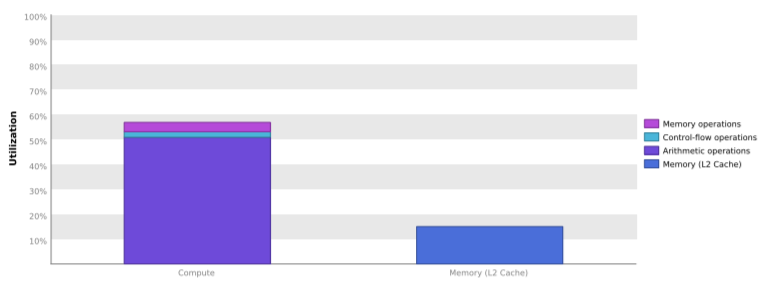
\includegraphics{contents/pics_1/nvvp_gpu.PNG}
    \caption{Kernel performance of \texttt{gpu2}.}
    \label{fig:nvvp_gpu}
\end{figure}

\noindent From figure \ref{fig:nvvp_gpu} above it is evident that too much time is spend on memory. This is quite surprising since matrix-matrix multiplication should be compute-bound for large problem sizes and not memory-bound. The \texttt{nvvp} profiler reveals that only 20 registers are used, while others (e.g. Hans Henrik) were able to use 32 registers. This automatically results in too many cache-misses since the 20 registers cannot store as much information, and hence memory has to be fetched more often. Therefore, time that could be spend on computing is instead spend on waiting for the memory to be loaded.\\

\noindent Unfortunately it was not clear what caused this low number of registers and how it could be increased, and therefore the issue could not be solved in time.\\

\noindent Similar problems occurred for the other versions: for \texttt{gpu3} the number of registers is 24, for \texttt{gpu4} the number is 27, and for \texttt{gpu5} the number of registers is 32. Even though the number of registers increased for each version, too much time was still spend on memory. It is possible that the new driver (which was not used due to time issues) would solve this problem. Another idea would be to run the driver on a different node.\\

\noindent A second suggestion for further improving the kernels applies to all of the different versions. Every single time an element of $A$ is multiplied by an element of $B$, global memory is accessed (by updating the corresponding element of $C$) which is very time consuming. This could be solved by using a local variable inside the kernel instead. I.e. if a local variable \texttt{C\_value} was used to store the intermediate value of the current element of $C$, it would only be necessary to access global memory once for each element of $C$ instead of every time an element of $A$ is multiplied by an element of $B$.\\

\noindent The implementation of version 5 actually uses a local variable inside the kernel, and this probably explains some of the extra speed-up compared to the other versions.

\newpage
\section{Poisson problem}
This section includes several algorithms/kernels, results and analysis of those performances. 
The performance of the kernel setups will be compared and they have been evaluated for $N = 2048$ and \texttt{max\_iter} = $1000$. The chosen parameters gives the refrence algorithm a runtime of $\approx1.5$ secound.

\noindent The main purpose of this section is to find the speedup for difference GPU implementations in reference of the best OpenMP (\texttt{jac\_cpu}) version from previous assignment. The environment variable which determines the wait policy of the threads has not been set to \texttt{OMP\_WAIT\_POLICY=active} is in the previous assignment. The OpenMP is evaluated with \texttt{OMP\_NUM\_THREADS=12}.
The achieved speedups are presented in table \ref{tab:speedup_pos}.

\noindent It has been chosen to validate the implementation of the difference GPU kernels by visualizing their estimates of $u(x,y)$ after the last iteration. This give a visual verfication of the kernel and source implementations. See plots in figure \ref{fig:apped_vis_pos} in the appendix.

\noindent The iterative process is controlled by the host and it uses \texttt{cudaDeviceSynchronize()} to make sure the work of the threads on the devices is done before incrementing the iteration. The iterative process \texttt{while(k < max\_iter)} which includes pointer switchs and new kernel calls is identical for all three GPU versions. Although the kernels are called by different 
kernel launch parameters: \texttt{<<<grid,block>>>}.

\noindent The initialization of the boundary conditions in $u$ and $u\_old$, and of the heating source given by $f$ are done on the on the host. The and copied to the device by using the approiate cuda calls.  
The I/O duration for transferring the initial matrices to the device and the duration of the transferring the estimate of $u$ back to host is included in the total compute time in order to make a fair comparison to the \texttt{jac\_cpu} function.



\subsection{Sequential GPU Jacobi}
The kernel used in the Sequential Poisson is provided in algorithm \ref{alg:jac_v1}. 

\noindent \texttt{jac\_gpu1} is called by the following launch parameters \texttt{<<<1,1>>>jac\_gpu1}. This ensures it only enables one block with one thread. See algo. \ref{alg:app_jac_v1} for the complete source code.

\lstinputlisting[label={alg:jac_v1},caption={Algo. \texttt{jac\_gpu1}.},style=CStyle, linerange={23-33}]{code_3/jac_gpu1.cu}.

\subsection{Naive GPU Jacobi}
The Naive Poisson kernel have been implemented by using one thread per grid point which enables the high parallelism of the device. The implementation uses global memory and line 2-3 shows how the upadted element is determined. The kernel is presented in algo. \ref{alg:jac_v2}.

\lstinputlisting[label={alg:jac_v2},caption={Algo. \texttt{jac\_gpu2}.},style=CStyle, linerange={24-31}]{code_3/jac_gpu2.cu}. 


\noindent The kernel is called by following launch paramters: \texttt{<<<dim\_grid,dim\_block>>>jac\_gpu2} which creates a 2D thread blocks. The 2D grid and block size are given by:
\begin{align}
dim3 \quad &dim\_grid \left(  \frac { N+bs-1 }{ bs },\frac { N+bs-1 }{ bs } \right)  \\
dim3\quad  &dim\_block\left(bs, bs \right)
\end{align}
where $bs=16$ is the number of threads in each block.


\subsubsection{\texttt{nvvp}}
The \texttt{nvvp} analyzing tool tells that the \texttt{jac\_gpu2()} has a "Low Compute Utilization" $\approx 16\%$, presented in figure \ref{fig:computebound}. This is as expected, as all memory is fetched globally in the implementation, and as only few floating point operations are performed every time memory is retrieved. Due to this difficulty, the Jacobi method is memory bound. This could be optimized by splitting up the copying, such that the algorithm could copy and compute simultaneously and hereby reduce the computation time. By using more specialized analysis tools within \texttt{nvvp}, a bandwidth limitation is proposed. This limits also supports the claim that the problem is memory bound.  The solution to the Poisson problem using this algorithm is presented in \ref{fig:jac_gpu2} in the appendix.\\

\begin{figure}[H]
\centering
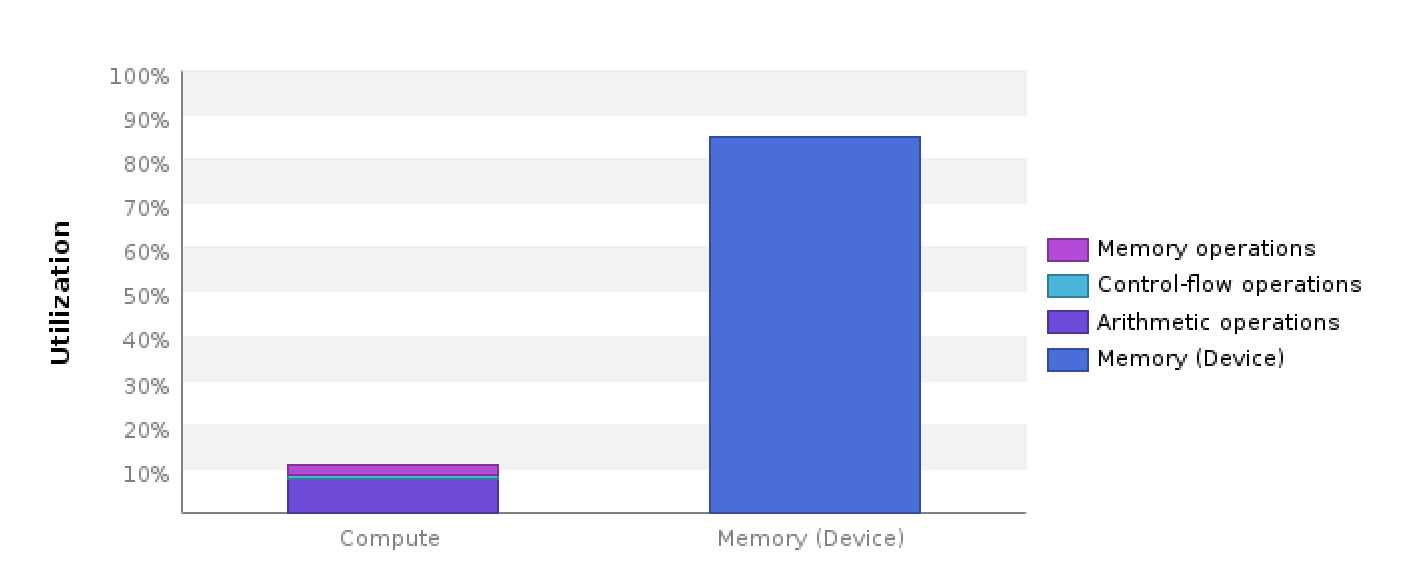
\includegraphics[width=1\textwidth]{data_3/pos_sceenshots/computebound.png}
\caption{The \texttt{nvvp} analysis of \texttt{jac\_gpu2()}. This reports that the algorithm is memory bound as the percentage of utilized memory is much bigger than the utilization of the computation.}
\label{fig:computebound}
\end{figure}

%Vi bruger lang tid på at copiere data, dette kunne blive forbredet hvis man kun kopierede lidt over af gangen . low compute utilization (16\%) pga lang tid om at kopiere. N = 2048, 1000 iterationer. low kernel concurrency.  



\subsection{Multiple GPU Jacobi}
The third version the Jacobi version use multiply (two) GPUs. The problem is hereby split equally between the devices. It has been chosen to create a horizontal split.

\noindent The kernels, \texttt{jac\_gpu3}, used to solve the Poisson problem is presented in algorithm \ref{alg:jac_v3_alg}. 

\noindent The \texttt{cudaDeviceEnablePeerAccess()} method is used to solve the boarder issues between the top and bottom problem as the Jacobi iteration uses the adjacent grid points when updating an element. See the complete source implementation, algo. \ref{alg:app_jac_v3} in the appendix.

\lstinputlisting[label={alg:jac_v3_alg},caption={Algo. \texttt{jac\_gpu3}.},style=CStyle, linerange={26-46}]{code_3/jac_gpu3.cu}

\noindent The kernel is, as in \texttt{jac\_gpu2}, called by the following launch paramters: \texttt{<<<dim\_grid,dim\_block>>> jac\_gpu3}. Noticeable the grid is $N/2$ in the second axis in order to support the dimensions of the each subproblem. The 2D grid and block size are given by:
\begin{align}
dim3 \quad &dim\_grid \left(  \frac { N+bs-1 }{ bs },\frac { N/2+bs-1 }{ bs } \right)  \\
dim3\quad  &dim\_block\left(bs, bs \right)
\end{align}



\subsection{Speedup}
The expected compute speedup is 8x\footnote{PerformanceTuningIntro.pdf, slide 20.} when deploying the algorithm on the GPU compared to the CPU.
Table \ref{tab:speedup_pos} reports the achieved speedups for the three implementations.

\begin{table}[!th]
\centering
\begin{tabular}{l|r}
Algo. & Speedup \\\hline
\texttt{cpu}&1.0000x \\
\texttt{gpu1}&0.0021x \\
\texttt{gpu2}&10.3818x \\
\texttt{gpu3}&16.5419x \\

\end{tabular}
\caption{This table present the speed-ups of \texttt{jac\_gpu1}, \texttt{jac\_gpu2} and, \texttt{jac\_gpu3} in reference to the fastest CPU version from assignment 2, \texttt{cpu()} }
\label{tab:speedup_pos}
\end{table}

\noindent As expected the \texttt{jac\_gpu1} does not gain any improvements. The reason why is the lack of parallelism. Hence there is only launched one block with one kernel.

\noindent The speedup gained by \texttt{jac\_gpu2} is $\approx 10x$ which slightly higher than the expected compute speedup. This can be caused by a version of the OpenMP implementation, which is not fully optimized. If the implementation is sub-optimal the comparison is not fair to the fully parallel implementation on the GPU.

\noindent When splitting the problem into two subproblems the expected speedup is \underline{not} $2x$ between \texttt{jac\_gpu2} and \texttt{jac\_gpu3}. The reason is due to the nature of the Jacobi algorithm. There needs to be shared global memory access between the two devices in order to update the "middle" horizontal boarders elements. The shared global memory, accessed by peer access, is transferred on the PCIe express bus which introduce a latency and therefore not able to scale $2x$. 

% \begin{figure}[H]
% \centering
% \begin{tikzpicture}[scale = 1]
% \begin{axis}[
%     width=10cm, height=8cm,     % size of the image
%     ybar,
%     %symbolic x coords={},
%     xticklabels={\texttt{jac\_cpu},\texttt{jac\_gpu1},\texttt{jac\_gpu2},\texttt{jac\_gpu3}},
%     xtick=data,
%     ytick={0,1,2,9,10,11,15,16,17},
%     ylabel=x,
%     %xlabel=Algo,
%     ]
    
% \addplot table [x=x, y=speed, col sep=comma]{data_3/performance_pos.txt};
    
% %\addplot table[x=interval,y=carT]{\mydata};
% \end{axis}
% \end{tikzpicture}
% \caption{Caption}
% \label{fig:speedup_pos}
% \end{figure}





\newpage
\section{Conclusion}
In the part concerning matrix-matrix multiplication, the analysis shows that there is a significant performance gain in using GPUs. used in \texttt{lib} to four. It is especially seen how shared memory improves the performance by considering \texttt{gpu2} and \texttt{gpu5}. Both algorithms uses one thread pr element in $C$, but the performance of \texttt{gpu5} is much higher, as the algorithm takes advantage of shared memory. The measured speed-ups might be overestimated due to using a driver, that limits the number of threads. If the updated driver had been used, the performance of \texttt{lib} might have been much better. Regarding the implementation of the algorithms, the \texttt{nvvp} profiler analysis showed that relatively few registers are used pr. thread. This limits the performance, as a lot of time is used on copying memory back and forth. This alone was not enough to explain the amount of time used on memory on the device, why it was discovered that every time an addition was made to an element in $C$, this was stored and fetched from the global memory. The kernels could have been optimized by saving the element of $C$ locally while computing it and then writing it to the global variable \texttt{d\_C}. \\
The experimentally achieved speed-ups reported table \ref{tab:speedup_pos} indicates a very good reason for performing this scientific computing problem on a many core multiprocessor such as a GPU or multiply GPUs compared to a traditional multi core CPU using a single treads pr. core.
The enhancement by performing the Jacobi algorithm on the GPU is $\approx 10x$. Splitting the problem into two subproblems scales further to $\approx 16x$.